\documentclass[a4paper]{article}
\usepackage[T1]{fontenc}
\usepackage[russian]{babel}
\usepackage[pdftex]{graphicx}
\usepackage[ruled,vlined]{algorithm2e}
\usepackage[utf8]{inputenc}
\usepackage{xcolor}
\usepackage{hyperref}
\usepackage{amsmath}
\usepackage{geometry}
\usepackage{float}
\usepackage{caption}
\usepackage{subcaption}
\DeclareGraphicsExtensions{.pdf,.png,.jpg}


\begin{document}

    \begin{titlepage}
        \Large
        \begin{center}
            Санкт-Петербургский \ Политехнический университет Петра Великого\\
            \vspace{10em}Отчет по лабораторной работе №7\\
            \vspace{2em}
            \textbf{Определение систематического сдвига в данных}
        \end{center}
        \vspace{6em}
        \hfill\parbox{10cm}{
            \hspace*{2cm}\hspace*{-4cm}Студент:\hfill Швачко Никита Андреевич\\
            \hspace*{2cm}\hspace*{-4cm}Преподаватель:\hfill Баженов Александр Николаевич\\
            \hspace*{2cm}\hspace*{-4cm}Группа:\hfill 5030102/20202
        }
        \vspace{\fill}
        \begin{center}
            Санкт-Петербург \ 2025
        \end{center}
    \end{titlepage}
    \section{Постановка задачи}
    Цель лабораторной работы — определить систематический сдвиг между двумя выборками с помощью индекса Жаккара для твинов (двойных интервалов). 
    Для этого были сгенерированы две выборки \( X_1 \) и \( X_2 \), обладающие различными средними и стандартными отклонениями:
    \[
        X_1 = N(0, 0.95), \quad X_2 = N(1, 1.05)
    \]
    Задача заключалась в том, чтобы варьировать параметр сдвига \( a \) таким образом, чтобы найти оптимальное значение, 
    при котором индексы Жаккара для твинов достигают максимума. Для каждой выборки были рассчитаны два типа твинов:
    \begin{itemize}
        \item Внутренний твин: \(\left[Q_{1/4}, Q_{3/4}\right]\) — первый и третий квартили
        \item Внешний твин: \(\left[\min X_i, \max X_i\right]\) — минимальное и максимальное значение выборки
    \end{itemize}
    Твин представляет собой двойной интервал вида \(X = [a,b] = [[a,a],[b,b]]\), где \(a\) и \(b\) — концы интервала.
    В результате работы были найдены оценки сдвига \( a \), при которых индексы Жаккара \( J_{\text{Inn}}(a) \) и \( J_{\text{Out}}(a) \) 
    достигают максимума.

    \section{Описание используемых методов}
    Для решения задачи был использован следующий подход:
    \begin{enumerate}
        \item \textbf{Генерация выборок}: С использованием библиотеки NumPy были сгенерированы две выборки \( X_1 \) и \( X_2 \) 
        по нормальному распределению с заданными параметрами.
        \item \textbf{Расчет твинов}: Для каждой выборки были рассчитаны два типа твинов:
        \begin{itemize}
            \item Внутренний твин (25\% и 75\% квантили)
            \item Внешний твин (минимум и максимум)
        \end{itemize}
        Твин представляет собой двойной интервал, где каждый конец является интервалом вида \([a,a]\).
        \item \textbf{Индекс Жаккара}: Для определения степени схожести выборок использовался индекс Жаккара, который вычисляется как:
        \[
        \begin{aligned}
        J_{\text{Inn}} & = \frac{\text{Inn } X_1 \wedge \text{Inn } X_2}{\text{Inn } X_1 \vee \text{Inn } X_2}, \\
        J_{\text{Out}} & = \frac{\text{Out } X_1 \wedge \text{Out } X_2}{\text{Out } X_1 \vee \text{Out } X_2},
        \end{aligned}
        \]
        где \(\wedge\) и \(\vee\) — операции минимума и максимума по включению соответственно.
        \item \textbf{Определение сдвига}: Параметр сдвига \( a \) изменялся в диапазоне от -2 до 4, и для каждого значения сдвига 
        рассчитывались индексы Жаккара для обоих типов твинов. Искались значения \( a \), при которых эти индексы 
        достигают максимума:
        \[
        \begin{aligned}
        a_{\text{Inn}} & = \arg\max_a J_{\text{Inn}}(a), \\
        a_{\text{Out}} & = \arg\max_a J_{\text{Out}}(a).
        \end{aligned}
        \]
        \item \textbf{Визуализация}: Для представления результатов были построены графики зависимостей индексов Жаккара от значения 
        сдвига, а также гистограммы распределений выборок с отмеченными твинами и их центрами.
    \end{enumerate}

    \section{Результаты эксперимента}
    В результате эксперимента были получены следующие данные:

    \begin{itemize}
        \item \textbf{Статистические характеристики выборок}:
        \begin{itemize}
            \item Выборка \(X_1\): \(\mu \approx 0.018\), \(\sigma \approx 0.930\)
            \item Выборка \(X_2\): \(\mu \approx 1.074\), \(\sigma \approx 1.047\)
            \item Теоретическая разница средних: \(1.000\)
        \end{itemize}

        \item \textbf{Твины для выборки X2}:
        \begin{itemize}
            \item Внутренний твин: \([[0.363, 0.363], [1.765, 1.765]]\)
            \item Длина внутреннего твина: \(1.402\)
            \item Центр внутреннего твина: \(1.064\)
            \item Внешний твин: \([[-2.087, -2.087], [4.353, 4.353]]\)
            \item Длина внешнего твина: \(6.440\)
            \item Центр внешнего твина: \(1.133\)
        \end{itemize}

        \item \textbf{Оценки сдвига}:
        \begin{itemize}
            \item Оценка сдвига для внутреннего твина: \( a_{\text{Inn}} \approx 0.990 \)
            \item Оценка сдвига для внешнего твина: \( a_{\text{Out}} \approx 0.709 \)
            \item Отклонение от теоретического значения для внутреннего твина: \(0.010\)
            \item Отклонение от теоретического значения для внешнего твина: \(0.291\)
        \end{itemize}

        \item \textbf{Твины при оптимальном сдвиге}:
        \begin{itemize}
            \item Внутренние твины:
            \begin{itemize}
                \item X1 (со сдвигом 0.990): \([[0.375, 0.375], [1.606, 1.606]]\)
                \item X2: \([[0.363, 0.363], [1.765, 1.765]]\)
                \item Индекс Жаккара: \(0.878\)
            \end{itemize}
            \item Внешние твины:
            \begin{itemize}
                \item X1 (со сдвигом 0.709): \([[-2.370, -2.370], [4.369, 4.369]]\)
                \item X2: \([[-2.087, -2.087], [4.353, 4.353]]\)
                \item Индекс Жаккара: \(0.956\)
            \end{itemize}
        \end{itemize}

        \item \textbf{Графики}: На графиках отображены зависимости индексов Жаккара от значения сдвига \( a \) и распределения 
        выборок с отмеченными твинами и их центрами. Максимальные значения индексов Жаккара соответствуют значениям сдвига 
        \( a_{\text{Inn}} \) и \( a_{\text{Out}} \) соответственно.
        \begin{figure}[H]
            \centering
            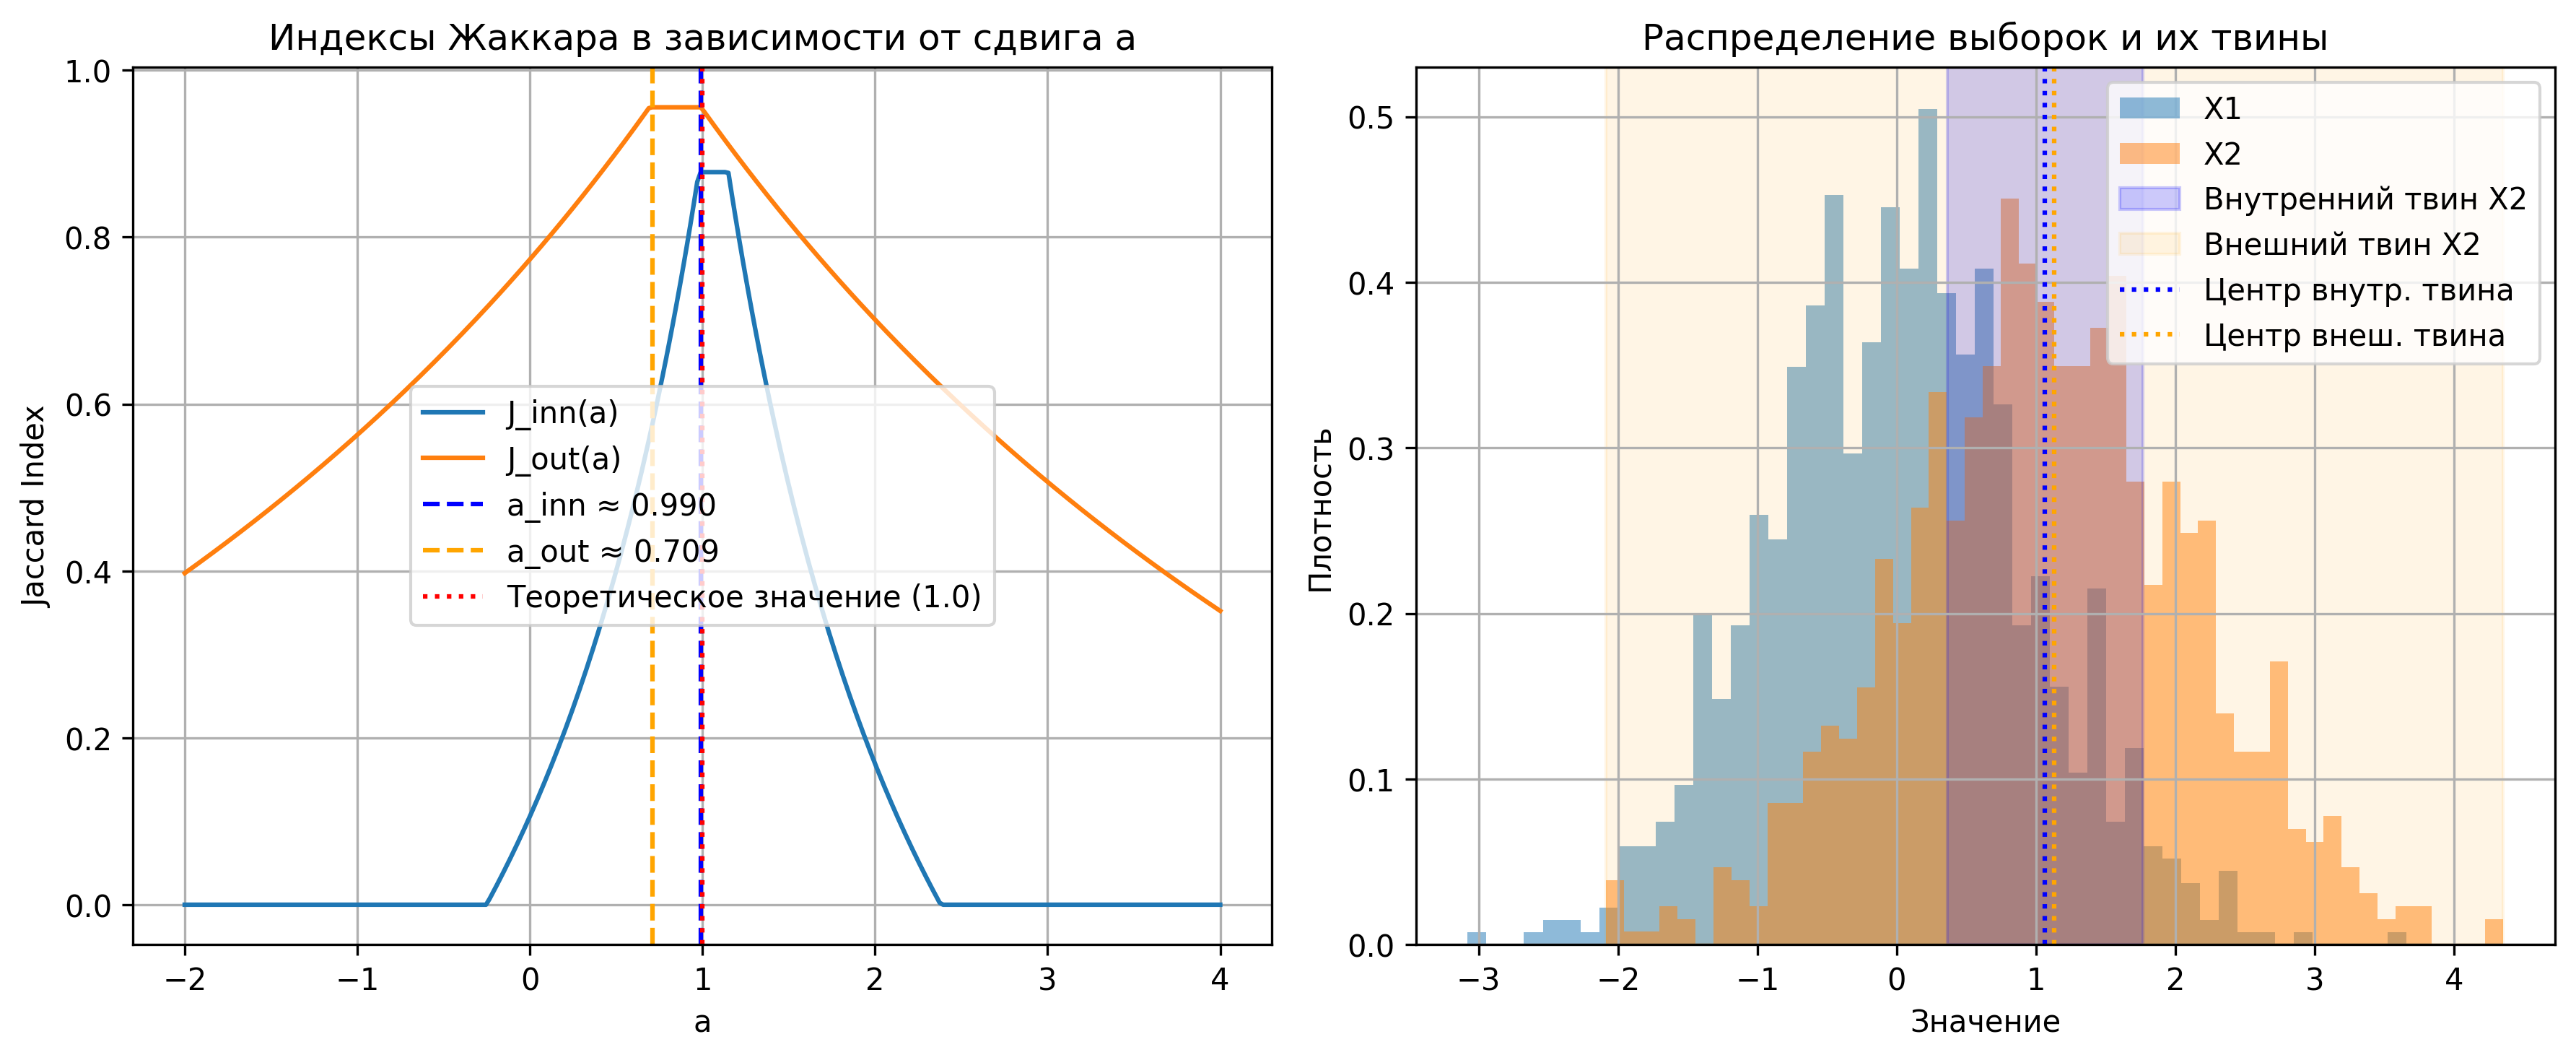
\includegraphics[width=1\textwidth]{plot}
            \caption{Зависимость индексов Жаккара от параметра сдвига \(a\) и распределение выборок с твинами}
        \end{figure}
    \end{itemize}

    \section{Выводы}
    В ходе лабораторной работы были исследованы изменения индексов Жаккара при варьировании сдвига между выборками,
    что позволило точно оценить параметры сдвига \( a \). Полученные результаты показывают, что:

    \begin{itemize}
        \item Метод внутреннего твина дал точную оценку сдвига (\(a_{\text{Inn}} \approx 0.990\)), 
        которая практически совпадает с теоретическим значением (отклонение всего \(0.010\)).
        \item Метод внешнего твина оказался менее точным (\(a_{\text{Out}} \approx 0.709\)), 
        что может быть связано с большей чувствительностью к выбросам.
        \item Использование твинов позволяет получить более полное представление о структуре данных, 
        так как каждый твин представляет собой двойной интервал, учитывающий как внутреннюю, так и внешнюю оценку.
        \item Центры твинов могут служить дополнительными характеристиками для анализа распределения данных.
        \item Индекс Жаккара для внешних твинов (\(0.956\)) оказался выше, чем для внутренних (\(0.878\)), 
        что говорит о большей степени перекрытия внешних интервалов при оптимальном сдвиге.
    \end{itemize}

\end{document}